\begin{frame}
\frametitle{Use $\times$ to find vector perpendicular to two given}
Recall $\textbf{u} \times \textbf{v}$ is perpendicular to $\textbf{u}$ and $\textbf{v}$.
\begin{example}
Find a vector perpendicular to $\textbf{u} =\langle1,1,0\rangle = \textbf{i}+\textbf{j}$ and $\textbf{v}=\textbf{j}+\textbf{k}=\langle 0,1,1 \rangle$:

\[
\begin{array}{rcl}
 \textbf{w} &= & (\textbf{i}+\textbf{j}) \times (\textbf{j}+\textbf{k}) =
\textbf{i} \times \textbf{j} + \textbf{i} \times \textbf{k} +
\textbf{j} \times \textbf{j} + \textbf{j} \times \textbf{k} = \\
& = & \textbf{k} -\textbf{j}+\textbf{0}+\textbf{i} = \textbf{i} - \textbf{j} + \textbf{k} = \langle1,-1,1\rangle\; .
\end{array}
\]
\end{example}
\end{frame}

\begin{frame}
\frametitle{Use $\times$ to find area of triangle in space}
\begin{columns}
\column{0.3\textwidth}
  \psfrag{u}{$\textbf{v}$}
  \psfrag{v}{$\textbf{u}$}
  \psfrag{w}{$\textbf{w}$}
    \psfrag{A}{$A$}
    \psfrag{B}{$B$}
    \psfrag{C}{$C$}
    \psfrag{D}{$D$}
  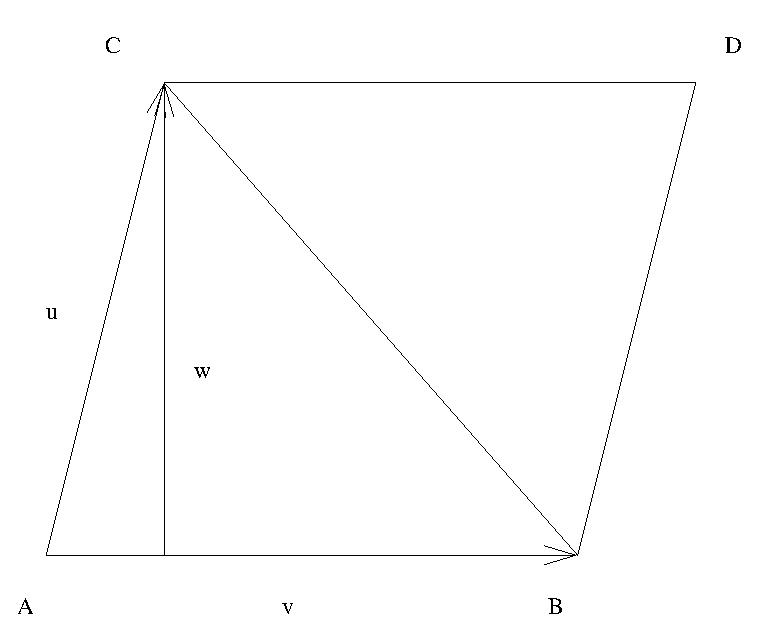
\includegraphics[height=1in]{../../modules/vectors/pictures/ok-area_triangle.eps}
\column{0.7\textwidth}
\begin{itemize}
\item $A$, $B$, $C$ points in space, $\textbf{u} = \textbf{AB}$, $\textbf{v}=\textbf{AC}$. 
\item Then $|\textbf{w}| = |\textbf{orth}_{\bm{u}} \textbf{v}| = \text{ distance from } C \text{ to } AB\; .$
\item $|\textbf{u} \times \textbf{v}| = |\textbf{orth}_{\bm{u}} \textbf{v}| \, |\textbf{u}| =
2 \text{area}(ABC) = \text{area}(ABDC)$
\item $|\textbf{u} \times \textbf{v}|$ = Area of parallelogram on sides $\textbf{u}$ and $\textbf{v}$.
\end{itemize}
%
\end{columns}
\end{frame}

\begin{frame}
\begin{example}
\begin{columns}
\column{0.3\textwidth}
\psset{xunit=0.7cm, yunit=0.7cm}
\begin{pspicture}(-0.1, -0.1)(4,4)
\fcBoundingBox{-0.2}{-1}{4}{3.5}
\fcAxesIIId{3}{3}{3}%
\pscustom*[linecolor=cyan]{%
\fcPolyLineIIId{[1 2 3] [2 3 1] [3 1 2] [1 2 3]}
}
\end{pspicture}
\column{0.7\textwidth}

Find the area of the triangle $A(1,2,3)$, $B(2,3,1)$, $C(3,1,2)$.

\end{columns}
\[\begin{array}{rcl}
\displaystyle \text{Area}(ABC) &=&\displaystyle \frac{1}{2}|\textbf{AB} \times \textbf{AC}| =
\frac{1}{2}|\langle 1,1,-2\rangle \times \langle 2, -1, -1\rangle | \\~\\
&=&\displaystyle\frac{1}{2} |\langle -3, -3, -3 \rangle| \\~\\
&=&\displaystyle \frac{3\sqrt{3}}{2}\; .
\end{array}
\]

\end{example}
\end{frame}